\documentclass[]{spie}  %>>> use for US letter paper
%\documentclass[a4paper]{spie}  %>>> use this instead for A4 paper
%\documentclass[nocompress]{spie}  %>>> to avoid compression of citations

\renewcommand{\baselinestretch}{1.0} % Change to 1.65 for double spacing
 
\usepackage{amsmath,amsfonts,amssymb}
\usepackage{graphicx}
\usepackage[colorlinks=true, allcolors=blue]{hyperref}

\title{Lynx grating spectrometer design: Optimizing chirped gratings}

\author[a]{Hans Moritz G\"unther}
\author[a,b]{Ralf K. Heilmann}
\affil[a]{MIT Kavli Institute for Astrophysics and Space Research, Massachusetts Institute of Technology, Cambridge, MA 02139, USA}
\affil[b]{Space Nanotechnology Laboratory, Massachusetts Institute of Technology, Cambridge, MA 02139, USA}

\authorinfo{Send correspondence to H.M.G. (E-mail: hgunther@mit.edu)}

% Option to view page numbers
\pagestyle{empty} % change to \pagestyle{plain} for page numbers   
\setcounter{page}{301} % Set start page numbering at e.g. 301
 
\begin{document} 
\maketitle

\begin{abstract}
Lynx is one of four concept studies for NASA's 2020 decadal survey. The design reference mission includes an X-ray grating spectrometer (XGS) based on critical angle transmission (CAT) gratings. In the past we studied different grating sizes and arrangements using traditional flat CAT gratings with constant bar spacing. However, new technology development brings chirped gratings in reach. Using chirped gratings where the grating bar spacing varies over a grating allows us to fill the aperture with larger gratings because the chirp can compensate for some aberrations caused by the deviation of large flat gratings from the Rowland torus. This reduces the area blocked by grating support structures. Using larger gratings also carries potential cost savings.
We use ray-tracing to study an XGS design with chirped grating to derive alignment tolerances and maximal size of the gratings used to stay within the Lynx requirements for effective area and resolving power. We find that using chirped gratings of $80 * 160$~mm size allows us to reduce the number of gratings from over 5000 to about 500, while simultaneously increasing the effective area by 25\% and keeping the resolving power constant.

\end{abstract}

% Include a list of keywords after the abstract 
\keywords{ray-tracing, X-ray, Lynx, CAT (critical angle transmission), spectroscopy}

\section{INTRODUCTION}
\label{sec:intro}
High resolution X-ray spectroscopy is a well-established method to study a wide variety of phenomena in the high-energy universe from early phases of star formation to the outflows of massive black holes in the center of far away galaxies. Often, high-resolution X-ray spectroscopy can reveal information than cannot be obtained by any other method. For example, the density of the accretion shock in young stars can only be measured in He-like triplets of O~{\sc vii} and Ne~{\sc ix}, located around 21 and 13~\AA{}, respectively. Despite great advances in X-ray microcalorimeters, only diffraction gratings can deliver a resolving power $> 1000$ in the soft X-ray band.

In preparation for the 2020 Decadal survey, NASA organized a detailed study of four surveyors-type missions, one of them focussed on the X-ray band, called ``Lynx''\cite{gaskin}. The design
reference mission (DRM) for Lynx includes a mirror with a 2~m$^2$ collecting area at
1~keV and a Point-spread-function (PSF) of 0.5~arcsec half-power-diameter
(HPD). Lynx would have two instruments at the focal point with different field-of-view and energy resolution (High-Definition X-ray Imager
(HDXI)\cite{HDXI} or microcalorimeter\cite{MICROCAL}) and tractable gratings that can be inserted into the beam to diffract photons to a separate detector (X-ray grating spectrometer - XGS). While reflection gratings have been considered\cite{OPXGS}, they are fundamentally limited in resolving power\cite{2020ApJ...897...92D} and the DRM relies on critical angle transmission (CAT) gratings.

The design, hardware requirements, and predicted performance of the XGS in the DRM is described in detail in Ref.~\citenum{CATXGS}; in the same reference we also explain the setup of our ray-trace simulations. In section~\ref{sect:raytrace} we present a short summary of the setup, but refer the reader to Ref.~\citenum{CATXGS} for more details. 

The goal of this paper is to study a scenario in detail that was only briefly mentioned in Ref.~\citenum{CATXGS}: CAT gratings with a ``chirp'', i.e.\ a spatially variable grating period $d$. We discuss the motivation to use chirped gratings in section~\ref{sect:motivation} before we go into results for ray-traces with chirped gratings (section~\ref{sect:chirp}). In principle, one could combine a chirp with physically bending the gratings, but we demonstrate in section~\ref{sect:bend} that the added benefit is small and does not justify the added complexity. We end with a summary in section~\ref{sect:summary}.

\section{SETUP FOR RAY-TRACES}
\label{sect:raytrace}
Our simulations are based on a geometric ray-trace, which follows
individual rays through the system from the entrance aperture to the
detector. Simulations are performed with MARXS
1.2\cite{marxs,marxs1.2}, which is written in Python and lincensed
under the GNU license v3. It is available on
github\footnote{\url{https://github.com/chandra-marx/marxs}}. Code specific to the Lynx XGS and the analysis shown in this article is also available\footnote{\url{https://github.com/hamogu/marxs-lynx}}; we
used the version with commit hash 13b10be. 

The setup is described in detail in Ref.~\citenum{CATXGS}. In addition, improvements on the treatment of the grating support structures, which act as diffraction gratings themselves, are described in \cite{10.1117/12.2525814}. For the analysis here, we assume that the parameters of the grating bar support structures do not depend on the size of the grating, i.e.\ that larger gratings do not require any thicker support structures than we assumed for the $50*50$~mm gratings discussed in Ref.~\citenum{CATXGS}.

The CAT gratings for the Lynx XGS are developed at the
MIT Space Nanotechnology Laboratory
\cite{Heilmann:11,doi:10.1117/12.2188525,10.1117/12.2314180,10.1117/12.2529354}. The high aspect-ratio grating bars are
5.7~$\mu$m deep and supported by an L1 support structure running
perpendicular to the grating bars themselves and the entire membrane
(bars and L1) is mechanically stabilized by a hexagonal L2 support
structure, which is 0.5~mm deep. 
A preliminary structural analysis indicates that changes in the shape of the L1 and L2 support structures could actually be used to reduce the thickness and covering fraction of the support structures compared to the current design, so our assumption that the L1 bars and L2 hexagons currently planned work for larger gratings as well seems reasonable for this early stage of the spectrograph design.
Absorption and diffraction of photons
by the L1 and L2 support structures is included in our
simulations. The grating membrane is surrounded by a narrow solid Si frame. We also explore if bending the gratings into the shape of a cylinder (with the axis of the cylinder parallel to the grating bars) can further improve performance. Smaller gratings with bars 4.0~$\mu$m deep and side of $10 * 30$~mm have been bend in the laboratory and where found to maintain grating efficiency with no obvious mechanical damage\cite{10.1117/12.2274205}.

\section{Motivation for chirped gratings}
\label{sect:motivation}
In the XGS, the diffraction gratings need to be arranged on the surface or a torus, the Rowland torus\cite{beuermann:78}. The Rowland torus is curved, but transmission gratings are usually flat. Thus, for any positioning of gratings, parts of the grating will be above and others below the Rowland torus surface. If a ray intersects with a grating too early, the ray will be diffracted at a larger distance from the focal plane and thus will land further away from the zeroth order, while rays intersecting a grating below the surface of the Rowland torus are diffracted not as far. This effect spreads out the photons and reduces the spectral resolving power. In earlier X-ray instruments with transmission gratings, e.g.\ the Chandra/HETG, this is not a limiting effect. Gratings are small (about 20~mm or so on the side) and the resolving power requirements are relatively modest compared with Lynx. However, for the Lynx X-ray grating spectrograph (XGS) this is actually an effect that can limit resolving power and drives the choice of grating size in the baseline design.

Different approaches can be used to compensate the loss in resolving power. The simplest idea might be to just use smaller gratings. Gratings of $20*50$~mm are small enough to match Lynx resolvng power requirements\cite{CATXGS}. However, several thousand gratings are needed to cover the aperture in this case. A second idea is to bend the gratings so that they are not flat and follow the torus better. So, in priciple curved gratings can be used to match the grating position better to the Rowland torus. This is complicated by the fact that we also try to maintain a narrow range of blaze angles to optimize the number of photons diffracted into grating orders which are covered by detectors. The radius of the Rowland circle is about half of the focal distance. To maintain the ideal blaze angle for all rays in a converging beam, the gratings would have to be bent with a radius close to the focal length, while the radius to match the surface of the torus is half of that. To make matters worse, in CAT (critical angle transmission) gratings, the gratings bars must be inclined with repect to the incoming rays. The structure of the silicon crystal and the CAT grating manufacturing process require that the gratings bars are perpendicular to the surface of the grating. In order to maintain a blaze angle around 1.6~degrees, gratings have to be mounted with an angle, adding further restrictions on bending them.

So, another appraoch is to use flat gratings, oriented to make the blaze condition work at least for the center ray, and to change the grating period $d$ smoothly over the grating ("chirp") such that the part of the grating that is located "below" the surface of the Rowland torus, where photons would be diffracted not far enough, has a slightly smaller $d$ and thus diffract to larger angles. Conversely, the part of the grating located "above" the Rowland torus needs to have a slightly larger $d$. The grating equation gives the relation between $\lambda$, the wavelength of the photon, the grating order $n$, and the angle of diffraction $\theta$:
$$
n\lambda = d \sin \theta \; .
$$

\section{Chirped gratings in the XGS}
\label{sect:chrip}
\subsection{General setup}
The baseline design for the Lynx XGS uses gratings of $20 * 50$~mm, where the long direction is perpendicular to the dispersion and is chosen to minimze technical risk, as this size of close to the sie of gratings that have been manufactured in the past. The short side is along the dispersion direction and is limited by the aberration discussed above. At this size, over 5000 gratings are required to cover the aperture. For most of the aperture, larger gratings of $50*50$~mm are also sufficient\cite{CATXGS}. So, with the added complexity of having gratings of two different sizes, the number of gratings can be brought down to about 3000. In contrast, we here investigate much larger gratings of $60 * 180$~mm. At this size, only about 500 gratings are required to cover the full aperture. The choice of $60 * 180$~mm is driven by the size of commercially available 200~mm waivers, such that one grating fits onto a waiver with comfortable margin for handling and processing.

In the following simulations, we assume a continous detector with no chip gaps. This is just a computational simplification, such that we can run simulations for just three wavelength points without worrying if any one of them falls into a chip gap.

Ray-racing is run with $10^5$ rays per simulation.


\subsection{Approach to find the chirp}
We chose a reference energy in the middle of the XGS bandpass (0.6~keV). 
For each grating, we calculate the position on the detector, where a ray that passes through the center of the grating intersects with the detector. For all other positions on the detector, we can then determine which diffraction angle $\theta$ is required to bring rays to the same position on the detector. From the grating equation, we can determine the value of $d$ required at that grating position. The 3D geometry of this is a litte cumbersome, so for simplicity we optimize $d$ numerically instead of tracing the geometry analytically. Numerically, we just perform the ray-trace varying $d$. Since we perform a ray-trace anyway, this is simple and fast to implement.

Of course, the diffraction of light requires a periodic structure and would not work if gratings did not have a regular period. However, the required chirp is so small that the period $d$ changes noticably only over macroscopic scales, thus diffraction still occurs. This is somewhat analogous to stacking a telescope with a large number of smaller gratings. The grating bars are periodic within each grating, but the gratings are not phased up, and diffraction still happens, as evidenced by the Chandra/HETGS and other observatories.

In principle, the chirp in $d$ is not the same for all wavelength and all angles, but since CAT gratings diffract photons into a relatively narrow range of angles, that is not a problem in practice, as we show below.

\begin{figure} [ht]
\begin{center}
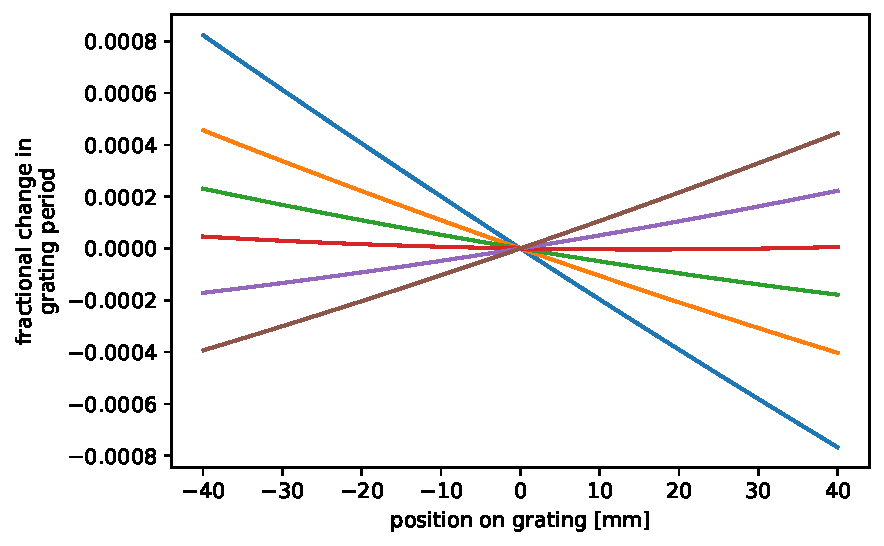
\includegraphics[width=0.7\textwidth]{chirps}
\end{center}
\caption {\label{fig:chirps}
Relative change in the grating period (chrip), that is required to a sample of XGS CAT gratings. The chirps are calcualted numerically for 50 evenly spaced points on each grating.
}
\end{figure}


Figure~\ref{fig:chirps} shows the relative change in the grating period for different gratings as calculated numerically. The gratings are located at different locations on the aperture. Some of them need a decreasing grating period in the direction of the positive $y$-axis, other require an increasing period. What they have in commmon though, is that all solutions are very close to linear. Thus, from now on, we will impose a linear relationship between the position on the grating and the fractional change in period. This speeds up the calculations significantly, because only a single point is needed to define a line that goes through 0 at the center of the ratings. Beyond numerical convenience, this also simplifies the specification of actual phyiscal gratings. While a different gradient in grating period $d$ might be needed for different gradients, all chirps have a linear relationship.


\subsection{How many different types of gratings do we need?}

The ideal chirp is different for every single grating. However, from a cost and schedule perspective, it is much preferrable to use only few different types of gratings. We can manufacture gratings with a few different chirps and then for each position pick a chirp that is very close to the ideal number. This deviation will lead to some loss of resolving power, but this is acceptable to a certain degree. While the simulations here are done with a perfectly aligned model, in practice, mechanical misalginments, aberations, and pointing errors all reduce the theoretically achievable resolving power. A small contribution from using grating with non-ideal chirps does not impact the final resolving power significantly.

In this section, we test how many different chirps are needed. We assume that there will always be  a group of gratings with no chirp. For example, a simulation might use gratings with just three different chirps: -0.0004, 0, 0.0004. Here the value of the chirp is expressed as the relative change of the grating period from the center to one edge. The relative change in $d$ for chirps of -0.0004 and +0.0004 is the same, just in one case it is increasing from left to right, in the other case, it is decreasing. CAT gratings do not have a preferred direction and the same type of grating can be used, just mounted with a different rotation, such that three values of the chirp can be realized with just two different physical gratings (or, e.g., five values of the chirp with just three types of grating, one with constant $d$ and two with different chirps). In practice, grating facets will have some handling layer, screw holes for mounting or similar, so that this has to be taken into account in the mechnical design, but this is still simpler than manufacturing, testing, etc.\ more different grating types.
Figure~\ref{fig:chirps_distribution} shows the ideal chirp (top left) for all gratings in the aperture, as well as the distribution of chirps for arrangements that use only 2, 3, or 5 different chirps. The required chirp depends soly on the position of the grating in dispersion directions, so the arrangement forms bands in the image. 

\begin{figure} [ht]
\begin{center}
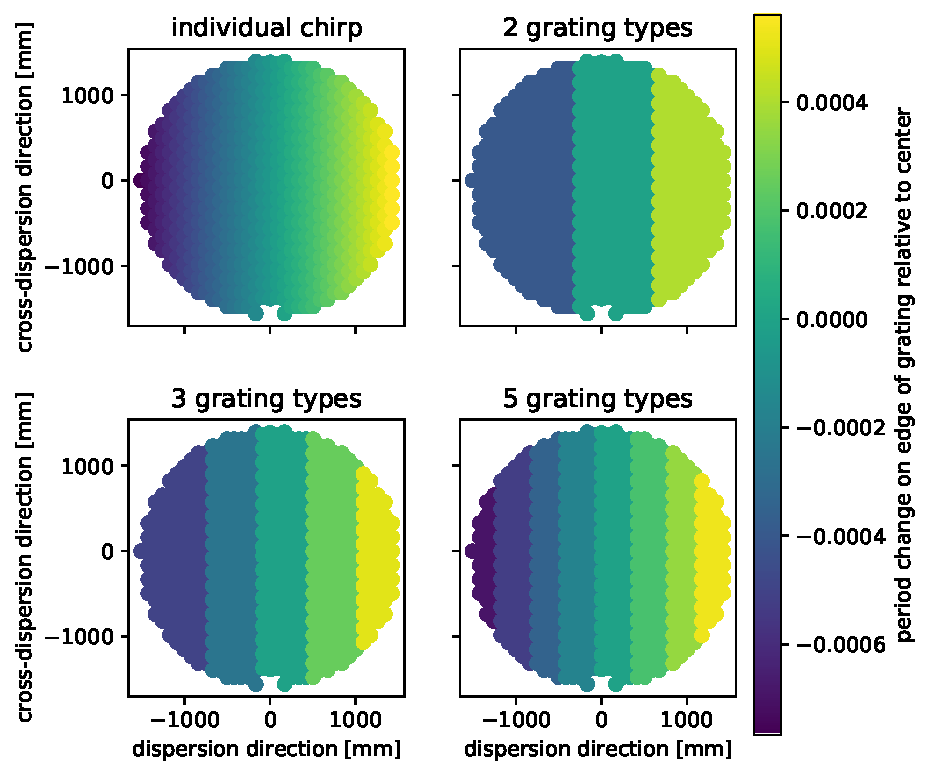
\includegraphics[width=0.7\textwidth]{chirps_distribution}
\end{center}
\caption {\label{fig:chirps_distribution}
This figure shows the distribution of chirps for different simulations. \emph{top left:} Gratings have individual chirps. \emph{other panels:} Setups with a limited number of grating types where for each position a chrip is chosen that is as close to the ideal chirp at that position as available. Assuming gratings can be reversed, two different chirps ($0, c$) allow for three different values ($-c, 0, c$) in the figure. Note that gratings do not touch each other, but at this scale the space between them is hard to see in the figure.

}
\end{figure}


\begin{figure} [ht]
\begin{center}
\includegraphics[width=0.7\textwidth]{chirps_aeff_res}
\end{center}
\caption {\label{fig:chirps_aeff_res}
 Resolving power (left) and effective area (right) for different grating arrangements. The resolving power $R$ given is averaged over all dispersed order, weighted by the signal in each order. Simulations are performed for three energies, spanning the XGS bandpass. 
}
\end{figure}

Figure~\ref{fig:chirp_aeff_res} shows the resolving power $R$ and effective area $A_{\mathrm{eff}}$ for those four scenarios, as well as the DRM baseline with smaller gratings and, for comparison, $160 * 80$~mm gratings with no chirp. 
The baseline scenario matches the Lynx requirements on $R$ and effective area, although a significant fraction of the aperture is covered by the frames and holders located around the grating membrane. For the baseline scenario, essentially the entire aperture needs to be filled with gratings to reach the requirement on $A_{\mathrm{eff}}$. The right plot shows that the effective area increases by about 20\% when larger gratings are used. The exact number depends on the distribution of the gratings over the aperture, the position of the mirror support spider, the size of the grating holders, the mounting strucutre etc., which can be optimized at a later stage, but it is clear evne fomr this simple model that larger gratings offer a better $A_{\mathrm{eff}}$, while simultaneously being more cost-effective because far fewer elements need to be manufactured, tested, and installed. The increased $A_{\mathrm{eff}}$ can either be used to improve the science output, or, for constant $A_{\mathrm{eff}}$ compared to the baseline design, we could subaperture, increasing $R$ over the number shown in the figure and reducing the number of gratings needed even further. 

In all cases, the chirp is calculated for photons of 0.6 keV, but for the angles and diffraction orders relevant for the XGS, the chirp is equally effective for all relevant energies.


\section{Should chirped gratings be bend?}
\label{sect:bend}

\section{Summary}
\label{sect:summary}
The grating size for the Lynx XGS is actually limited by the aberrations introduced by finite sized, flat gratings. A spectral resolving power $R$ of order 5000 can only be achieved with gratings no larger than about $20 * 50$~mm$^2$, if covereing the full aperture, or $50 * 50$~mm$^2$ if sub-aperturing is used such that the areas of the aperture where the departure from the Rowland torus is largest remain free form gratings. For Lynx, a few thousand gratings are needed to cover the aperture. We show here that chirped gratings can be used at much larger sizes, so that only a few hundred gratings are needed. The optimal chirp is different for every grating position, but filling the aperture with gratings with just five different chirps still matches the resolving power requirement of Lynx. Given other non-ideal effects, such as mechanical alignment, using five different chirps is sufficient that the accuracy of the chirp is no longer the limiting factor for the system resolving power.
We also investigated gratings that are bend and chirped, but found little added benefit.

\acknowledgments % equivalent to \section*{ACKNOWLEDGMENTS}
Support
for this work was provided in part through NASA grant NNX17AG43G and
Smithsonian Astrophysical Observatory (SAO) contract SV3-73016 to MIT
for support of the {\em Chandra} X-Ray Center (CXC), which is operated
by SAO for and on behalf of NASA under contract NAS8-03060.  The
simulations make use of Astropy, a community-developed core Python
package for Astronomy\cite{astropy1,astropy2}, numpy\cite{numpy}, and
IPython\cite{IPython}. Displays are done with mayavi\cite{mayavi} and
matplotlib\cite{matplotlib}.


% References
\bibliography{report} % bibliography data in report.bib
\bibliographystyle{spiebib} % makes bibtex use spiebib.bst

\end{document} 
